\documentclass[../main.tex]{subfiles}
\begin{document}
\clearpage
\section{Выпуклость множеств достижимости квазилинейных систем с интегральными ограничениями на управление}
This paper investigates convexity of reachable sets for quasilinear systems under integral quadratic constraints. Drawing inspiration from B.\,T.~Polyak's work on small Hilbert ball image under nonlinear mappings, the study extends the analysis to scenarios where a small nonlinearity exists on the system's right-hand side. At zero value of a small parameter, the quasilinear system turns into a linear system and its reachable set is convex.  The investigation reveals that to maintain convexity of reachable sets of these systems, the nonlinear mapping's derivative must be Lipschitz continuous. The proof methodology follows a Polyak's scheme. The paper's structure encompasses problem formulation, exploration of parameter linear mapping and image transformation, application to quasilinear control systems, and concludes with illustrative examples. 

\subsection{Введение в раздел}

Предметом исследования в этом разделе являются множества достижимости квазилинейных систем с интегрально-квадратичными ограничениями.

Исследование восходит к работам Б.\,Т.~Поляка\cite{Polyak2001}, в которых были получены достаточные условия выпуклости нелинейного отображения малого гильбертова шара.
These conditions were further applied to problems in control theory, demonstrating that the reachable set of a nonlinear system exhibits convexity given a sufficient small control resource, provided that the linearized system is controllable. A series of papers \cite{GusOsSteklov, GusevUMJ, Osipov, GusOsUdmurt} used the convexity conditions of the small ball mapping to investigate the reachable sets of nonlinear systems under integral constraints over small time intervals. 
In this case, it is important to note that the controllability of the linearized system alone does not guarantee convexity of the reachable sets for the nonlinear system. Additional conditions related to the asymptotic behavior of the eigenvalues of the controllability Gramian of the linearized system need to be imposed.  Once these conditions are fulfilled, the reachable sets of the nonlinear system not only exhibit convexity but are also asymptotically equivalent to the reachable sets of the linearized system.

Therefore, the study investigates the convexity of reachable sets of nonlinear systems with something small: with a small control resource and on a small time interval. This paper discusses another, third, variant of convexity of reachable sets of systems with a small parameter, namely with a small nonlinearity on the right hand side.

Systems that have small nonlinearity on the right-hand side are commonly called quasilinear systems.
The study of such systems in control theory dates back to the 1960s \cite{Subbotin, Kiselev, Kras_book}.
E.\,G.~Albrecht solved several problems concerning quasilinear systems \cite{Albrecht3}, including the optimal motion problem \cite{Albrecht1} and the game problem of quasilinear objects rendezvous\cite{Albrecht2}.
Control problems for quasilinear systems are also addressed in the following works \cite{Dauer, Kremlev, KalininLavrinovich2018, Gabasov}.
In modern applications of control theory, quasilinear systems arise after feedback linearization \cite{Calvet} and
stochastic linearization \cite{Ching, Gui}.

This paper studies the convexity of the reachable sets of quasilinear systems under integral constraints. 
In line with the papers \cite{Polyak2001, Polyak2004, GusOsSteklov, GusevUMJ, Osipov, GusOsUdmurt}, the study is reduced to the analysis of a non-linear mapping from the  control space and the small parameter space to the space of the trajectories endpoints generated by these controls.
In this case, the reachable set is the image of the ball under this mapping. 
The specific feature of the mapping defined by the solution of a quasilinear system is the fact that, at zero value of the small parameter, this mapping becomes linear in control.
For the image of the ball to preserve its convexity for small values of the small parameter, it is necessary for the nonlinear part of the mapping to have a Lipschitz  continuous derivative. 
The proof scheme for this statement is quite similar to the proof scheme for the main theorem in \cite{Polyak2001}.

The following is the paper's structure. The problem statement and some remarks are given in the second section. The third section contains the investigation of parameter linear mapping and image of a ball. In next section, we apply the results of the third section to the quasilinear control system. Finally, we provide two illustrative examples in the fifth section.

\subsection{Постановка задачи и предварительные замечания}


Further we use the following notation. By $A^{\top}$ we denote the transpose of a real matrix $A$, $I$ is an identity matrix, $0$ stands for a zero vector or a zero matrix of appropriate dimension. 
%For $x,\ y \in \mathbb{R}^n $ let $(x,y)=x^{\top}y$ denotes the inner product of two vectors, $x = (x_1,\dots,x_n)$, $\|x\| = (x,x)^{\frac{1}{2}}$ be the Euclidean norm, and $ B_X(\overline{x},r)=\{x\in\mathbb{R}^n : \|x - \overline{x}\|\leqslant r\}$ is the ball in Hilbert space $X$ with radius $r>0$ centered at $x$.
For a real $n \times n$ matrix $A$ a spectral matrix norm induced by the Euclidean vector norm is denoted as $\|A\|$.
The symbols $\mathbb{L}_1$ and $\mathbb{L}_2$ stand for the spaces of summable and square summable functions respectively. The norms in these spaces are denoted as $\|\cdot\|_{\mathbb{L}_1}$ and $\|\cdot\|_{\mathbb{L}_2}$. By $B_X(a,r)$ we will denote the closed ball of radius $r>0$ centered at $a$, $B_X(a, r) = \{x\in X: \|x-a\|_X \leqslant r \}$. Here $X$ is some linear space with a norm $\|\cdot\|_X$.


Рассмотрим квазилинейную систему
\begin{gather}\label{sec3:nonlinear}
	\dot{x}(t) = A(t)x(t)+B(t)u(t)+\varepsilon f\big(x(t),t\big), \qquad t_0 \leqslant t \leqslant T, \qquad x(t_0) = x_0,
\end{gather}
где $ x \in \mathbb{R}^n $ --- вектор состояния, $ u \in \mathbb{R}^r $ --- вектор управления, $t_0$ --- неотрицательное число, $T$ --- положительное число, а $\varepsilon$ --- малый параметр, такой что $\varepsilon \in [0,\overline{\varepsilon}]$, $ \overline{\varepsilon} > 0$. Матричные отображения  $A:[t_0,T] \to \mathbb{R}^{n\times n} $, $B: [t_0,T] \to \mathbb{R}^{n\times r} $ предполагаются непрерывными. 
Вектор функция $f: \mathbb{R}^n \times [t_0,T] \to \mathbb{R}^n$ непрерывна по паре $(x,t)$ и непрерывно-дифференцируема по  $x$.

Управление $ u(\cdot) $ будем выбирать из шара $ B_{\mathbb{L}_2}(0,\mu) $ где $ \mu > 0$.

Каждому управлению $u(\cdot) \in \mathbb{L}_2$ и любому $\varepsilon \in [0,\overline{\varepsilon}]$ соответствует единственное абсолютное непрерывное решение $ x(t,\varepsilon, u(\cdot)) $ системы \eqref{sec3:nonlinear}, удовлетворяющее начальному условию $ x(t_0,\varepsilon, u(\cdot)) = x_0$, и это решение продолжимо на интервал $[t_0, t_0 + \Delta]$, где $t_0 + \Delta < T$. 

Далее, мы будем считать выполненными условия следующего предположения.

\begin{assumption}\label{as:right_hand_side_conditions}
	
	Существует такое $\overline{\mu} > \mu $ что для любого $\varepsilon \in [0, \overline{\varepsilon}] $ все решения $ x(t,\varepsilon, u(\cdot)) $ отвечающие управлениям $u(\cdot) \in B_{\mathbb{L}_2}(0,\overline{\mu})$  лежат в выпуклом компакте $D \subset \mathbb{R}^n$.
	Кроме этого, предполагается, что функция $f: \mathbb{R}^n \times [t_0,T] \to \mathbb{R}^n$ и ее производная по $x$ удовлетворяют условию Липшица с константами $L_f$ и $l_f$ соответственно
	\begin{gather*}
		\left\| f(x_1,t) - f(x_2,t) \right\| \leqslant L_f \left\| x_1 - x_2 \right\|, \quad t\in[t_0,T], \quad x_1, x_2 \in D\\
		\left\| \frac{\partial f(x_1,t)}{\partial x} - \frac{\partial f(x_2,t)}{\partial x} \right\| \leqslant l_f \left\| x_1 - x_2 \right\|, \quad t\in[t_0,T], \quad x_1, x_2 \in D.
	\end{gather*}
\end{assumption} 

В частности, первая часть Предположения \ref{as:right_hand_side_conditions} выполняется, если  $f$ удовлетворяет одному из следующих условий \cite{Fillipov2}:
\begin{gather}\label{sublinear_growth}
	\left\|f\big(x,t\big) \right\| \leqslant l_1(t) (1 + \|x\|), \\ 
	x \cdot f(x,t) \leqslant a(t) \|x\|^2 + b(t),
\end{gather}
где $l_1(\cdot) \in \mathbb{L}_1[t_0,T]$ и $a(\cdot), b(\cdot)$ --- некоторые непрерывные функции.

\begin{definition} 
	Множеством достижимости $G(T,\mu,\varepsilon) $ системы \eqref{sec3:nonlinear} в момент $T$ называется множество всех возможных состояний, в которые система может быть переведена  к моменту $T$ при помощи управлений  $ u(\cdot) \in B_{\mathbb{L}_2}(0,\mu) $.
	\begin{gather*}
		G(T,\mu,\varepsilon) =\{\widetilde{x}\in \mathbb{R}^n:\exists u(\cdot)\in B_{\mathbb{L}_2}(0,\mu),\; x(T,\varepsilon,u(\cdot)) = \widetilde{x}\}.
	\end{gather*}
\end{definition} 
Возникает вопрос, при каких условиях множество достижимости системы \eqref{sec3:nonlinear} будет сохранять выпуклость при малых $\varepsilon$?

\subsection{Нелинейное отображение с малым параметром}

В этом параграфе, $x$ (а также $x_0$, $x_1$ и другие) никак не связан с вектором состояния системы \eqref{sec3:nonlinear}.
Здесь $x$ --- это элемент пространства $X$, а вот $\varepsilon$ по-прежнему малый неотрицательный параметр.

Будем рассматривать отображение $F(x, \varepsilon) = a_0 + A_0x + \varepsilon A_1(x,\varepsilon): B_X(0, r) \times \mathbb{R}_+ \rightarrow Y$, где $X$ и $Y$ --- гильбертовы пространства.
Здесь $a_0 \in Y$ --- константа, которая не зависит ни от $x$ ни от $\varepsilon$, $A_0$ --- линейный оператор, который предполагается сюръективным отображением $X$ в $Y$. 
%It is assumed that for $\varepsilon = 0$ the mapping $F(x, 0)=A_0x$ is a continuous operator which is linear with respect to $x$ and is a surjective mapping from $X$ to $Y$. 
Из последнего следует, что существует такое $\nu > 0$, что

\begin{gather}\label{regular}
	\| A_0^*y\| \geqslant \nu \|y\|, \quad \forall y \in Y.
\end{gather}
Здесь $A_0^* $ --- сопряженный к$A_0$ линейный оператор.
Наконец,  $A_1: B_X(0, r) \times \mathbb{R}_+ \to Y $ --- это нелинейный оператор, непрерывный по $x$ и $\varepsilon$.
\begin{assumption}\label{as:derivative_of_A1}
	Существует такое $\overline{\varepsilon} > 0$, что для всех $x \in B_X(0,r)$, $\varepsilon \in [0, \overline{\varepsilon}]$ отображение $A_1(x, \varepsilon)$  имеет производную Фреше $\frac{\partial A_1(x, \varepsilon)}{\partial x} = A_1'(x, \varepsilon)$  которая непрерывна по $\varepsilon$ и липшицева по $x$: существует $L>0$, такая что
	\begin{gather*}
		\|A_1'(x_1,\varepsilon) - A_1'(x_2,\varepsilon) \| \leqslant L\|x_1-x_2\|, \qquad x_1, x_2 \in B_X(0,r), \qquad \varepsilon \in [0, \overline{\varepsilon}].
	\end{gather*}
\end{assumption}

Для дальнейших рассуждений нам потребуется процитировать результат из \cite{Polyak2001, Polyak1964}.  В формулировке следующей леммы предполагается, что $f:X \to Y$ --- это нелинейное отображение, имеющее производную Фреше.
\begin{lemma}[\cite{Polyak2001, Polyak1964}]\label{lem:Polyak_lemma}
	Пусть существуют такие $L$, $\rho$, $\mu > 0$ и $y_0 \in Y$, что 
	\begin{gather*}
		\| f'(x) - f'(z) \| \leqslant L \| x - z\|, \quad \forall x,z \in B(x_0,\rho), \\
		\| f'(x)^*y \| \geqslant \mu \|y \|, \quad \forall y \in Y, \quad \forall x \in B(x_0, \rho), \\
		\| f(x_0) - y_0 \| \leqslant \rho \mu,
	\end{gather*}
	тогда уравнение $f(x) = y_0$ имеет решение $x^* \in B(x_0,\rho)$ и 
	\begin{gather*}
		\|x^* - x_0\| \leqslant \frac{1}{\mu} \left\| f(x_0) - y_0 \right\|.
	\end{gather*}
\end{lemma}
Теперь мы можем сформулировать и доказать следующую теорему.
\begin{theorem}\label{th:ImageConvexity}
	Через $F(x,\varepsilon)$ обозначим образ шара $B_X(0, r)$ при его отображении $F\big(B_X(0,r),\varepsilon\big)$, т.е. $F\big(B_X(0,r),\varepsilon\big) = \big\{F(x,\varepsilon): x\in B_X(0, r)\big\}$.
	Пусть выполнено Предположение \ref{as:derivative_of_A1} и $F\big(B_X(0,r),\varepsilon\big)$ --- замкнутое множество для каждого  $\varepsilon \in [0, \overline{\varepsilon}]$. Тогда найдется такое $ \varepsilon_0 \in (0, \overline{\varepsilon}]$, что при всех положительных $\varepsilon < \varepsilon_0$ образ $F\big(B_X(0,r),\varepsilon\big)$ --- выпуклое множество в $Y$. 
\end{theorem}
\doc
Заметим, что константа $a_0$ не влияет на выпуклость образа $F\big(B_X(0,r),\varepsilon\big)$. 
Поэтому, в доказательстве, мы будем считать ее равной нулю.

Рассмотрим две произвольные точки, $x_1$ и $x_2$, из шара $B_X(0,r)$. 
Обозначим $x_0 = \frac{1}{2}(x_1 + x_2)$, $y(\varepsilon) = \frac{1}{2}\big(y_1(\varepsilon)  + y_2(\varepsilon)\big)$, где $y_1(\varepsilon) = F(x_1, \varepsilon)$ и $y_2(\varepsilon) = F(x_2, \varepsilon)$. 

Для того, чтобы доказать выпуклость множества $F\big(B_X(0,r),\varepsilon\big)$, достаточно показать, что $y(\varepsilon) \in F\big(B_X(0,r),\varepsilon\big)$ или, что тоже самое, найдется такое $x^* \in B_X(0,r) $, что $F(x^*, \varepsilon) = y(\varepsilon) $.
Выпишем выражение для $y(\varepsilon)$
\begin{gather}\label{y}
	\begin{gathered}
		y(\varepsilon)=
		\frac{1}{2} \big(
		F(x_1,\varepsilon)+ 
		F(x_2,\varepsilon)
		\big) = 
		\frac{1}{2} \big(
		A_0 x_1 +
		\varepsilon A_1(x_1,\varepsilon) +
		A_0 x_2 +
		\varepsilon A_1(x_2,\varepsilon) 
		\big) = \\ = A_0 x_0 + 
		\frac{1}{2} \varepsilon \big( 
		A_1(x_1,\varepsilon)+ 
		A_1(x_2,\varepsilon)
		\big).
	\end{gathered}
\end{gather}

Пусть $x \in X$ и $h \in X$ выбраны так, чтобы выполнялись включения $x\in B_X(0, r)$ и $x+h \in B_X(0, r)$.
В условиях Предположения \ref{as:derivative_of_A1}, разложим $A_1$ в ряд около точки $x$:

\begin{gather}\label{A1_series}
	A_1(x + h,\varepsilon) = A_1(x,\varepsilon) + A_1'(x,\varepsilon) h + R(\varepsilon, x, h).
\end{gather}

Умножив обе части равенства на $y^* \in Y^*$, $\|y^*\| \leqslant 1$ имеем
\begin{gather*}
	\langle y^*, R(\varepsilon, x, h) \rangle = 
	\langle y^*, A_1(x + h,\varepsilon) \rangle -
	\langle y^*, A_1(x,\varepsilon) \rangle -
	\langle y^*, A_1'(x,\varepsilon) h \rangle
\end{gather*}

Применив теорему о среднем к функции $\langle y^*, A_1(x,\varepsilon) \rangle$, получим
\begin{gather*}
	\langle y^*, A_1(x + h,\varepsilon) \rangle -
	\langle y^*, A_1(x,\varepsilon) \rangle = 
	\langle y^*, A_1'(x + \theta h,\varepsilon) h \rangle,
	\qquad
	0 \leqslant \theta \leqslant 1.
\end{gather*}

Два последних соотношения приводят нас к оценке
\begin{gather}
	\begin{gathered}
		\|\langle y^*, R(\varepsilon, x, h) \rangle \| \leqslant
		\| y^* \| 
		\| A_1'(x + \theta h,\varepsilon)  -
		A_1'(x,\varepsilon) \| 
		\| h  \| \leqslant 
		L \theta \|h\|^2 \leqslant
		L \|h\|^2, \\
		\| R(\varepsilon, x, h) \| \leqslant
		L \|h\|^2, 
	\end{gathered}
\end{gather}

Подставим \eqref{A1_series} в выражение для \eqref{y}

\begin{gather*}
	y(\varepsilon) =
	A_0x_0 +
	\frac{1}{2}\varepsilon \Big(
	A_1(x_0,\varepsilon) +
	A_1'(x_0,\varepsilon)(x_1 - x_0)+ 
	R(\varepsilon, x_0, x_1 - x_0) + \\ 
	A_1(x_0,\varepsilon) +
	A_1'(x_0,\varepsilon)(x_2 - x_0)+ 
	R(\varepsilon, x_0, x_2 - x_0)
	\Big) = \\ = 
	A_0x_0 + 
	\varepsilon A_1(x_0,\varepsilon) +
	\xi(\varepsilon,x_1,x_2).
\end{gather*}
где остаточный член может быть записан в форме
\begin{gather*}
	\xi(\varepsilon,x_1,x_2) = \frac{1}{2}\varepsilon\big(R(\varepsilon, x_0, x_1 - x_0) + R(\varepsilon, x_0, x_2 - x_0)\big),
\end{gather*}
и оценен через
\begin{gather*}
	\|\xi(\varepsilon,x_1,x_2)\| \leqslant \frac{1}{2}\varepsilon L \left(\frac{1}{4}\|x_1 - x_2\|^2 + \frac{1}{4}\|x_1 - x_2\|^2 \right) \leqslant \frac{1}{4}L\varepsilon\|x_1 - x_2\|^2.   
\end{gather*}

Таким образом, $y(\varepsilon) = A_0x_0 + \varepsilon A_1(x_0,\varepsilon) + \xi(\varepsilon,x_1,x_2) = F(x_0,\varepsilon) + \xi(\varepsilon,x_1,x_2)$ для всех $x_1, x_2 \in B(0,r)$, $x_1 \neq x_2$, $\varepsilon \in [0, \overline{\varepsilon}]$, а значит выполняется следующее неравенство
\begin{gather*}
	\| F(x_0,\varepsilon) - y(\varepsilon) \| = \|\xi(\varepsilon,x_1,x_2)\| \leqslant \frac{1}{4}L\varepsilon\|x_1-x_2\|^2.
\end{gather*}


Теперь рассмотрим производную $F(x_0, \varepsilon)$ по $x_0$ при фиксированном $\varepsilon$, $F_x'(x_0,\varepsilon) = A_0 + \varepsilon A_1'(x_0,\varepsilon) $.

Из предположения \ref{as:derivative_of_A1} мы можем оценить $\|A_1'(x_0,\varepsilon\|$ сверху:
\begin{gather*}
	\|A_1'(x_0,\varepsilon) - A_1'(0,\varepsilon)\| \leqslant 
	L\|x_0\| \leqslant
	L r, \\
	\|A_1'(x_0,\varepsilon)\|  \leqslant \| A_1'(0,\varepsilon)\| + Lr.
\end{gather*}

Из равенства $\|A_1'(x_0,\varepsilon)\| = \|\big(A_1'(x_0,\varepsilon)\big)^*\| $, следует, что  $\|\big(A_1'(x_0,\varepsilon)\big)^*\| \leqslant \| A_1'(0,\varepsilon)\| + Lr$.
Отсюда и из соотношения \eqref{regular}, мы получаем 
\begin{gather*}
	\left\|F'_x(x_0, \varepsilon)^* y\right\| = \left\|\big(A_0 + \varepsilon A_1'(x_0, \varepsilon)\big)^* y\right\| \geqslant \left\|A_0^*y \right\| - \varepsilon \left\|\big(A_1'(x_0,\varepsilon)\big)^*\right\| \left\|y\right\| \geqslant (\nu - k\varepsilon)\|y\|,
\end{gather*} где $k = \max\limits_{\varepsilon \in [0,\overline{\varepsilon}]}\| A_1'(0,\varepsilon)\| + Lr > 0$.
Для малых $\varepsilon$, выполняется следующее неравенство $(\nu - k\varepsilon) \geqslant \dfrac{\nu}{2}$ и мы получаем $\left\|F'_x(x_0, \varepsilon)^* y\right\| \geqslant \dfrac{\nu}{2} \|y\|$. Для того, чтобы использовать Лемму  \ref{lem:Polyak_lemma}, потребуем

\begin{gather*}
	\| F(x_0,\varepsilon) - y(\varepsilon) \| = \|\xi(\varepsilon,x_1,x_2)\| \leqslant \frac{1}{4}L\varepsilon\|x_1-x_2\|^2 \leqslant \dfrac{\nu}{2} \dfrac{\|x_1-x_2\|^2}{8r}.
\end{gather*}

Чтобы это неравенство выполнялось, значение  $\varepsilon$ должно удовлетворять $\varepsilon \leqslant \varepsilon_0 = \min\left\{\dfrac{\nu}{4Lr}, \dfrac{\nu}{2k}, \overline{\varepsilon}\right\}$. 

Наконец, из Леммы \ref{lem:Polyak_lemma} с параметрами $\mu=\dfrac{\nu}{2}$ и $\rho=\dfrac{\|x_1-x_2\|^2}{8r}$ следует, что существует такой $x^*\in B(x_0, \rho)$, что $F(x^*,\varepsilon) = y(\varepsilon)$.
Так как $B_X(0, r)$ --- гильбертов шар, строго выпуклое множество, то выполняется включение $B(x_0, \rho) \subset B_X(0, r)$, следовательно $x^* \in B_X(0, r)$. Таким образом, точка $y(\varepsilon) = \frac{1}{2} \big( F(x_1,\varepsilon) + F(x_2,\varepsilon)\big)$ лежит в образе шара $F\big(B_X(0,r),\varepsilon\big) $  при  всех  $\varepsilon \leqslant \varepsilon_0$ и $x_1, x_2 \in B_X(0,r)$. Из-за замкнутости, для всех $\varepsilon \leqslant \varepsilon_0$, образ шара$F\big(B_X(0,r),\varepsilon\big) $ будет выпуклым.
\hfill$\square$\\[1ex]%--- P r o o f.

\subsection{О свойства решений квазилинейных систем}
\setcounter{equation}{0}


В этом разделе исследуются решения \eqref{sec3:nonlinear} для того, чтобы обосновать применение результатов предыдущего раздела, а именно Теоремы \ref{th:ImageConvexity}. 

Обозначим фундаментальную матрицу системы $\dot{x}(t) = A(t) x(t)$ через $X(t,\tau)$.
Эта матрица является решением уравнения
\begin{gather*}
	\frac{\partial X(t,\tau)}{\partial t} = A(t) X(T,\tau), \qquad X(\tau,\tau) = I.
\end{gather*}

Если $x(\cdot,\varepsilon, u(\cdot))$ --- решение \eqref{sec3:nonlinear}, порожденное управлением $u(\cdot)$ и начальными условием $x_0$,  то оно удовлетворяет интегральному уравнению
\begin{gather*}
	x\big(T,\varepsilon, u(\cdot)\big) =
	X(T,t_0)x_0 + 
	\int\limits_{t_0}^T X(T,\tau) \bigg(Bu(\tau) +
	\varepsilon f\Big(x\big(\tau,\varepsilon, u(\cdot)\big),\tau\Big) \bigg)\ d\tau = \\ =
	X(T,t_0)x_0 +
	\int\limits_{t_0}^T X(T,\tau) B(t)u(\tau)\ d\tau 
	+ \varepsilon \int\limits_{t_0}^T X(T,\tau) f\Big(x\big(\tau,\varepsilon, u(\cdot)\big),\tau\Big) \ d\tau.
\end{gather*}

Определим отображение $F:B_{\mathbb{L}_2}(0,\overline{\mu})\times [0,\overline{\varepsilon}] \to \mathbb{R}^n$ равенством $F(u(\cdot),\varepsilon) = x(T,\varepsilon,u(\cdot))$, где $x(T,\varepsilon,u(\cdot))$ --- решение \eqref{sec3:nonlinear} в момент $T$ отвечающее управлению $u(\cdot)$ и малому параметру $\varepsilon$.

Для того, чтобы использовать результаты предыдущего раздела, перепишем  $F$ в виде
\begin{gather*}
	F(u(\cdot),\varepsilon) = a_0 + A_0 u(\cdot) + \varepsilon A_1(u(\cdot), \varepsilon), 
\end{gather*}
где $a_0 = X(T,0)x_0 $, а отображения $A_0: B_{\mathbb{L}_2}(0,\overline{\mu})  \mapsto \mathbb{R}^n$ и $A_1: B_{\mathbb{L}_2}(0,\overline{\mu}) \times [0,\overline{\varepsilon}] \to \mathbb{R}^n$ определены равенствами
\begin{gather}\label{A1_def}
	A_0 u(\cdot) = \int\limits_{t_0}^T X(T,\tau) B(t)u(\tau)\ d\tau, \qquad
	A_1(u(\cdot),\varepsilon) = \int\limits_{t_0}^T X(T,\tau) f\Big(x\big(\tau,\varepsilon, u(\cdot)\big),\tau\Big) \ d\tau.
\end{gather}

Множество достижимости $G(T,\mu,\varepsilon) $  квазилинейной системы \eqref{sec3:nonlinear} --- это образ шара $B_{\mathbb{L}_2}(0,\mu)$ при его отображении $F$, $G(T,\mu,\varepsilon) = F(B_{\mathbb{L}_2}(0,\mu),\varepsilon)$.

\begin{utv}\label{ReachableSetcloseness}
	Пусть выполнены условия Предположения \ref{as:right_hand_side_conditions}. Тогда, для всех $\varepsilon\in [0,\overline{\varepsilon}]$, множество достижимости $G(T,\mu,\varepsilon) $ --- замкнуто.
\end{utv}
\doc. 
Доказательство следует из равностепенной непрерывности траекторий, равномерной ограниченности траекторий и слабой компактности $B_{\mathbb{L}_2}(0,\mu)$ (см., например \cite{GusZyk}).
\hfill$\square$\\[1ex]%--- P r o o f.

Для того, чтобы применить Теорему \ref{th:ImageConvexity} к отображению $F$,  нам необходимо показать, что Предположение \ref{as:derivative_of_A1} выполняется для $A_1$, определенного в \eqref{A1_def}.
\begin{lemma}\label{lem:Lipx}
	Пусть выполнены условия Предположения \ref{as:right_hand_side_conditions}. Тогда, для всех $\varepsilon\in [0,\overline{\varepsilon}]$, найдется такая $L_x(\varepsilon) > 0$, что для любых $u_i(\cdot) \in B_{\mathbb{L}_2}(0,\mu), \ i = 1,2$ и $t \in [t_0,T]$, 
	\begin{gather*}
		\| x_1(t) - x_2(t) \| \leqslant L_x(\varepsilon) \| u_1(\cdot) - u_2(\cdot) \|_{\mathbb{L}_2},
	\end{gather*}
	где $x_i(t) = x(t,\varepsilon,u_i(\cdot))$, $i = 1,2$. Кроме того, $L_x(\varepsilon) \leqslant L_x(\overline{\varepsilon})$. 
\end{lemma}
\doc.
Так как $x_i(t) \in D$ для всех $t\in [t_0,T]$, из Предположения \ref{as:right_hand_side_conditions}, мы имеем
\begin{gather*}
	\|f\big(x_1(t),t\big) - f\big(x_2(t),t\big)\| \leqslant L_f\|x_1(t) -  x_2(t)\|.
\end{gather*}
Из интегрального соотношения
\begin{gather}\label{nonlinear_solution}
	x_i(t) = x_0 + \int\limits_{t_0}^t A(\tau)x_i(\tau)\ d\tau + \int\limits_{t_0}^t B(\tau)u_i(\tau)\ d\tau+
	\varepsilon\int\limits_{t_0}^t f\big(x_i(\tau),\tau\big)\ d\tau,
\end{gather}
мы имеем
\begin{gather*}
	\| x_1(t) - x_2(t) \| \leqslant
	\left\| \int\limits_{t_0}^t A(\tau)\big(x_1(\tau) - x_2(\tau)\big)\ d\tau \right\| + 
	\left\|\int\limits_{t_0}^t B(\tau) \big(u_1(\tau) - u_2(\tau)\big)\ d\tau   \right\| + \\ +
	\varepsilon \left\| \int\limits_{t_0}^t \Big( f\big(x_1(\tau),\tau\big) - f\big(x_2(\tau),\tau\big) \Big)\ d\tau   \right\|  
	\leqslant \\ \leqslant
	\int\limits_{t_0}^t \big(k_A + L_f \varepsilon) \left\| x_1(\tau) - x_2(\tau)\right\| \ d\tau + k_u \| u_1(\cdot) - u_2(\cdot) \|_{\mathbb{L}_2}.
\end{gather*}
Здесь, 
\begin{gather*}
	k_u = \sqrt{(T-t_0) \max\limits_{\tau \in [{t_0},t]}\|B(\tau)\|}, \quad k_A =\max\limits_{\tau \in [{t_0},t]} \| A(\tau)\|.
\end{gather*}
Из неравенства Гронуолла 
\begin{gather*}
	\| x_1(t) - x_2(t) \| \leqslant L_x(\varepsilon) \| u_1(\cdot) - u_2(\cdot) \|_{\mathbb{L}_2},
\end{gather*}
где $L_x(\varepsilon) = k_u \exp\big((k_A + L_f \varepsilon)(T - t_0)\big) $. Заметим, что $L_x(\varepsilon) \leqslant L_x(\overline{\varepsilon})$. 
\hfill$\square$\\[1ex]%--- P r o o f.



% To analyze the derivative of mapping $A_1$, we require a lemma about the differentiation of an integral mapping. The following result is similar to the one in the book\cite{Luenberger}, but with one distinction: the book provides it for a function from $\mathbb{C}$, while in our analysis, we require this fact for a function from $\mathbb{L}_2$.

% \begin{lemen}\label{LeibnizRule}\cite[p.~174]{Luenberger}
	%     Let $f: \mathbb{L}_2 \to \mathbb{R}^n$ be a nonlinear mapping, defined by $f(x(\cdot)) = \\ = \int_{t_0}^T g(x(t),t)\ dt$, where $g: \mathbb{L}_2 \times \mathbb{R} \to \mathbb{R}^n$ is mapping with Frechet derivative $g_x:\mathbb{L}_2 \times \mathbb{R} \to \mathbb{R}^n$, which is uniform continuous with respect to x and t. Then, the Frechet differential of $f$ is
	%     \begin{gather*}
		%         \delta f(x,\delta x(\cdot)) = \int\limits_{t_0}^T g_x(x(t),t) \delta x(t)\ dt.
		%     \end{gather*}
	% \end{lemen}
% \proofen  
% We have 
% \begin{gather*}
	%     \left\|f(x+\delta x) - f(x) - \delta f (x,\delta x)\right\| = \left\|\int\limits_{t_0}^T
	%     \Big(g\big(x(t)+\delta x(t),t\big) - g\big(x(t),t\big) - g_x\big(x(t),t\big)\delta x(t)\Big) \ dt\right\|
	% \end{gather*}
% For almost all fixed $t$ we have, by the mean value theorem,
% \begin{gather}\label{meanvalue}
	%     g\big(x(t)+\delta x(t),t\big) - g\big(x(t),t\big) = g_x\big(\overline{x}(t),t\big)\delta x(t),
	% \end{gather}
% where $\|x(t) - \overline{x}(t)\| \leqslant \|\delta x(t)\| $. 
% The left part of the equality \eqref{meanvalue} is measurable, therefore the right part is measurable as well.
% The uniform continuity of $g_x$ with recpect to $x$ implies
% \begin{gather*}
	%     \|g_x(\overline{x}(t),t) \delta x(t) - g_x(x,t) \delta x(t) \| \leqslant L_g \|x(t) - \overline{x}(t)\| \|\delta x(t)\| \leqslant  L_g \|\delta x(t)\|^2.
	% \end{gather*}
% Finally, we have
% \begin{gather*}
	%     \left\|f(x+\delta x) - f(x) - \delta f (x,\delta x)\right\| = \left\|\int\limits_{t_0}^T
	%     \Big( g_x\big(\overline{x}(t),t\big)- g_x\big(x(t),t\big)\Big)\delta x(t)\Big) \ dt\right\| \leqslant \\  \leqslant
	%     \int\limits_{t_0}^T \left\|
	%     \Big( g_x\big(\overline{x}(t),t\big)- g_x\big(x(t),t\big)\Big)\delta x(t)
	%     \right\| \ dt \leqslant 
	%     L_g \|\delta x(\cdot)\|_{\mathbb{L}_2}^2.
	% \end{gather*} 
% The result follows.
% \hfill$\square$\\[1ex]%--- P r o o f.

Введем отображение $\overline{F}: [t_0,T] \times [0,\overline{\varepsilon}] \times B_{\mathbb{L}_2}(0,\overline{\mu}) \to \mathbb{R}^n$, равенством $\overline{F}(\tau,\varepsilon, u(\cdot)) = x \big(\tau,\varepsilon, u(\cdot)\big) $, где $x \big(\tau,\varepsilon, u(\cdot)\big)$ --- это решение системы \eqref{sec3:nonlinear} в момент $\tau$ порожденное управлением $u(\cdot)$ и малым параметром  $\varepsilon$.  Производная Фреше этого отображения $\overline{F}$ по $u(\cdot)$, $\overline{F}': B_{\mathbb{L}_2}(0,\overline{\mu}) \to \mathbb{R}^n $ --- это решение линеаризованной системы, см., например \cite{GusZyk}
\begin{gather}\label{dF}
	\overline{F}'(\tau,\varepsilon, u(\cdot)) \delta u(\cdot) = \delta x(\tau), 
\end{gather}
где $\delta x(\tau)$ --- это решение системы \eqref{sec3:nonlinear}, линеаризованной вдоль $(u(\cdot),x(\cdot,\varepsilon, u(\cdot))$ и отвечающее управлению $\delta u(\cdot)$ и нулевым начальным условиям:
\begin{gather}\label{dx}
	\delta\dot{x} =   \overline{A}\big(t,\varepsilon,u(\cdot)\big) \delta x +  B(t)\delta u(t), \qquad 0\leqslant t \leqslant \tau, \qquad \delta x(0) = 0,
\end{gather}
где
\begin{gather*}
	\overline{A}\big(t,\varepsilon,u(\cdot)\big) = A(t) +\varepsilon \frac{\partial f\big(x(t,\varepsilon,u(\cdot)\big),t\big)}{\partial x}.
\end{gather*}
\begin{lemma}\label{lem:Lipdx}
	Пусть выполнено Предположение \ref{as:right_hand_side_conditions}.  Тогда найдется  $L_u(\varepsilon) > 0$ такая, что для всех $\varepsilon\in [0,\overline{\varepsilon}]$, $u_i(\cdot) \in B_{\mathbb{L}_2}(0,\mu)$ и $\tau \in [t_0,T]$, 
	\begin{gather*}
		\| \overline{F}'(\tau,\varepsilon, u_1(\cdot)) - \overline{F}'(\tau,\varepsilon, u_2(\cdot)) \| \leqslant L_u(\varepsilon) \| u_1(\cdot) - u_2(\cdot) \|_{\mathbb{L}_2},
	\end{gather*}
	где $i = 1,2$.
\end{lemma}
\doc. 
Решение \eqref{dx} имеем вид
\begin{gather}\label{xu}
	\delta x\big(\tau,\varepsilon,u_i(\cdot),\delta u(\cdot)\big) = \int\limits_{t_0}^{\tau}  \overline{X}(\tau,s,\varepsilon,u_i(\cdot)) B(s) \delta u(s) \ ds,
\end{gather}
где $X(\tau,s,\varepsilon,u(\cdot)) $ --- фундаментальная матрица системы \eqref{dx}, которая является решением уравнения
\begin{gather*}
	\frac{\partial \overline{X}(\tau,s,\varepsilon,u(\cdot))}{\partial s} = -\overline{A}\big(s,\varepsilon,u(\cdot)\big)^{\top} \overline{X}(\tau,s,\varepsilon,u(\cdot)), \quad \overline{X}\big(\tau,\tau,\varepsilon,u(\cdot)\big) = I.
\end{gather*}
Хорошо известно(например, это следует из доказательства Теоремы 3 из \cite{Fillipov}), что существует такая константа $k_X>0$ что
\begin{gather*}
	\| \overline{X}(\tau,s,\varepsilon,u(\cdot)) \| \leqslant k_X, \qquad \tau \in [t_0,T], \qquad s \in [t_0,T]
\end{gather*}
для всех $u(\cdot) \in B_{\mathbb{L}_2}(0,\mu)$ и достаточно малого $\varepsilon $. Для сокращения записи, обозначим $\overline{A}_i(t) = \overline{A}\big(t,\varepsilon,u_i(\cdot)\big) $ и $ \overline{X}_i(t,s) = \overline{X}(t,s,\varepsilon,u_i(\cdot))$. В условиях предположения \ref{as:right_hand_side_conditions} и используя Лемму \ref{lem:Lipx} мы можем получить оценку
\begin{gather*}
	\int\limits_{t_0}^{\tau} \|\overline{A}_1(s) - \overline{A}_2(s) \| ds \leqslant L_A \| u_1(\cdot) - u_2(\cdot) \|_{\mathbb{L}_2}. 
\end{gather*}
Здесь $L_A>0$ не зависит от $u_1(\cdot)$, $u_2(\cdot)$, $\tau$ и $\varepsilon$. Используя,
\begin{gather*}
	\frac{\partial}{\partial t} \left(\overline{X}_1(t,s) - \overline{X}_2(t,s) \right) = -\overline{A}_1^{\top}(t) \left(\overline{X}_1(t,s) - \overline{X}_2(t,s) \right) + (\overline{A}_2(t) - \overline{A}_1(t))^{\top} \overline{X}_2(t,s), \quad t \in [s,\tau]
\end{gather*}
мы приходим к
\begin{gather*}
	\overline{X}_1(\tau,s) - \overline{X}_2(\tau,s) = \int\limits_s^{\tau} Y(t,s) \big(\overline{A}_2(t) - \overline{A}_1(t)\big)^{\top} X_2(t,s) dt.
\end{gather*}
Здесь $Y(t,s)$ --- это фундаментальная матрица системы 
\begin{gather*}
	\dot{y} = -\overline{A}_1(t) y.
\end{gather*}
Как и $\overline{X}_i(\tau,s)$, эта матрица тоже ограниченна: существует $k_Y>0$ такая, что
\begin{gather*}
	\|Y(t,s)\| \leqslant k_Y, \quad t,s \in [t_0, \tau]
\end{gather*}
для всех $u(\cdot) \in B(0,\mu)$. Мы имеем
\begin{gather*}
	\| \overline{X}_1(\tau,s) - \overline{X}_2(\tau,s) \| \leqslant L_X \| u_1(\cdot) - u_2(\cdot) \|_{\mathbb{L}_2}, \quad \mbox{where} \quad L_X = k_Y L_A k_X (T - t_0) .
\end{gather*}
Отсюда и из \eqref{xu} следует утверждение Леммы и $L_u(\varepsilon) = L_X(\varepsilon)\tau $.
\hfill$\square$\\[1ex]%--- P r o o f.

Теперь перейдем к определению дифференцируемости Фреше отображения $A_1(u(\cdot),\varepsilon)$ по $u(\cdot)$.
Выберем произвольную $u(\cdot) \in B_{\mathbb{L}_2}(0,\mu)$ и $\delta u(\cdot)$, так чтобы $\|\delta u(\cdot)\|_{\mathbb{L}_2} \leqslant \overline{\mu}-\mu$ и рассмотрим разность
\begin{gather}\label{diff_A}
	A_1(u(\cdot) + \delta u(\cdot),\varepsilon) - A_1(u(\cdot) ,\varepsilon) = \int\limits_{t_0}^T X(T,\tau) \left[ 
	f\Big(x\big(\tau,\varepsilon, u(\cdot) + \delta u(\cdot)\big),\tau\Big) - 
	f\Big(x\big(\tau,\varepsilon, u(\cdot)\big),\tau\Big) \right]\ d\tau.
\end{gather}

Изучим подробнее разность между решениями \eqref{sec3:nonlinear}, порожденнными $u(\cdot)$ и $u(\cdot) + \delta u(\cdot)$. Из \eqref{nonlinear_solution} следует
\begin{gather}\label{diff_of_x}
	\begin{gathered}
		x\big(t,\varepsilon, u(\cdot) + \delta u(\cdot)\big) -
		x\big(t,\varepsilon, u(\cdot)\big) 
		= \int\limits_{t_0}^t A(\tau) \left[
		x\big(\tau,\varepsilon, u(\cdot) + \delta u(\cdot)\big) -
		x\big(\tau,\varepsilon, u(\cdot)\big) 
		\right]\ d\tau + \\ +
		\int\limits_{t_0}^t B(\tau) \delta u(\tau)\ d\tau +
		\varepsilon\int\limits_{t_0}^t \left[ 
		f\Big(x\big(\tau,\varepsilon, u(\cdot) + \delta u(\cdot)\big),\tau\Big) -
		f\Big(x\big(\tau,\varepsilon, u(\cdot)\big),\tau\Big)
		\right]\ d\tau.
	\end{gathered}
\end{gather}

Пусть $y \in \mathbb{R}^n$ и $h \in \mathbb{R}^n$ выбраны так, что выполнялись включения $y\in D$ и $y+h \in D$. Тогда, для всех $\tau \in [t_0,T]$, используя представление приращения функции через интеграл по параметру, мы имеем

\begin{gather*}
	f(y + h, \tau) - f(y,\tau) = 
	% \int\limits_{y}^{y+h} 
	% \frac{\partial f}{\partial x}  \big(x, \tau\big) dx = 
	\left( \int\limits_{0}^{1} 
	\frac{\partial f}{\partial x}  \big(y + \xi h, \tau\big)\ d\xi \right) h =
	\frac{\partial f}{\partial x}  \big(y, \tau\big) h + \omega(y,h,\tau),
\end{gather*}
где 
\begin{gather*}
	\omega(y,h,\tau) = \left( \int\limits_{0}^{1} 
	\left[\frac{\partial f}{\partial x}  \big(y + \xi h, \tau\big) -
	\frac{\partial f}{\partial x}  \big(y, \tau\big) \right] \ d \xi \right) h.
\end{gather*}

Так как $D$ выпукло, $ y + \xi h \in D$ для всех0 $\leqslant \xi \leqslant 1$.
Значит, используя Предположение \ref{as:right_hand_side_conditions},  мы можем получить следующую оценку
\begin{gather*}
	\|\omega(y,h,\tau)\| \leqslant l_f \left( \int\limits_0^1  \left\| \xi h \right\| \ d\xi \right)h  \leqslant \frac{l_f}{2} \|h\|^2.
\end{gather*}

Положив $y = x\big(\tau,\varepsilon, u(\cdot)\big)$  и $h = \Delta x\big(\tau, \varepsilon, \delta u(\cdot)\big) = x\big(\tau,\varepsilon, u(\cdot) + \delta u(\cdot)\big) - x\big(\tau,\varepsilon, u(\cdot)\big)$, для всех $\tau \in [t_0,T]$ мы получаем
\begin{gather}\label{mean-value}
	\begin{gathered}
		f\Big(x\big(\tau,\varepsilon, u(\cdot) + \delta u(\cdot)\big),\tau\Big) -
		f\Big(x\big(\tau,\varepsilon, u(\cdot)\big),\tau\Big) = \\ = 
		\frac{\partial f}{\partial x}  \Big(x\big(\tau,\varepsilon, u(\cdot)\big), \tau\Big) 
		\Delta x\big(\tau, \varepsilon, \delta u(\cdot)\big)  + 
		\omega\Big(x\big(\tau,\varepsilon, u(\cdot)\big),\Delta x\big(\tau, \varepsilon, \delta u(\cdot)\big),\tau\Big),
	\end{gathered}
\end{gather}
где (см. Лемму \ref{lem:Lipx})
\begin{gather}\label{omega_est}
	\left\|\omega\Big(x\big(\tau,\varepsilon, u(\cdot)\big),\Delta x\big(\tau, \varepsilon, \delta u(\cdot)\big),\tau\Big)\right\| 
	\leqslant
	\frac{l_f}{2} \left\|\Delta x\big(\tau, \varepsilon, \delta u(\cdot)\big)\right\|^2 
	\leqslant
	\frac{l_f}{2} L_x^2(\overline{\varepsilon}) \|\delta u(\cdot)\|_{\mathbb{L}_2}^2.
\end{gather}
% where $\overline{x}(\tau) \in [x\big(\tau,\varepsilon, u(\cdot), x\big(\tau,\varepsilon, u(\cdot) + \delta u(\cdot)\big)]$ for all $\tau \in [t_0, T]$, so  $\|\overline{x}(\tau) - x\big(\tau,\varepsilon, u(\cdot)\big)\| \leqslant \|x\big(\tau,\varepsilon, u(\cdot) + \delta u(\cdot)\big) - x\big(\tau,\varepsilon, u(\cdot)\big)\|$. 

Из \eqref{mean-value} следует, что $\omega\Big(x\big(\tau,\varepsilon, u(\cdot)\big),\Delta x\big(\tau, \varepsilon, \delta u(\cdot)\big),\cdot\big)$ измерима, как сумма измеримых функций.
Подставляя \eqref{mean-value} в \eqref{diff_of_x}, получаем
\begin{gather*}
	\Delta x\big(t, \varepsilon, \delta u(\cdot)\big)
	= \int\limits_{t_0}^t 
	\overline{A}\big(\tau,\varepsilon,u(\cdot)\big) 
	\Delta x\big(\tau, \varepsilon, \delta u(\cdot)\big)\ d\tau + 
	\int\limits_{t_0}^t B(\tau) \delta u(\tau)\ d\tau + \\ +
	\varepsilon\int\limits_{t_0}^t \omega\Big(x\big(\tau,\varepsilon, u(\cdot)\big),\Delta x\big(\tau, \varepsilon, \delta u(\cdot)\big),\tau\Big) d\tau = 
	\delta x(t) + \Omega(t,\varepsilon, \delta u(\cdot)),
\end{gather*}
где $\delta x(t)$ --- это решение системы \eqref{dx} и
\begin{gather*}
	\Omega(t,\varepsilon, \delta u(\cdot)) = \varepsilon\int\limits_{t_0}^t 
	\omega\Big(x\big(\tau,\varepsilon, u(\cdot)\big),\Delta x\big(\tau, \varepsilon, \delta u(\cdot)\big),\tau\Big) d\tau
\end{gather*}


Поскольку \eqref{omega_est} мы можем оценить $\Omega(t,\varepsilon, \delta u(\cdot)) $ сверху для всех $t \in [t_0, T]$
\begin{gather}
	\| \Omega(t,\varepsilon, \delta u(\cdot))\| \leqslant \frac{l_f}{2} \overline{\varepsilon} L_x^2(\overline{\varepsilon})(T-t_0)\|\delta u(\cdot)\|_{\mathbb{L}_2}^2.
\end{gather}

Теперь мы можем переписать \eqref{mean-value} в виде,  
\begin{gather*}
	f\Big(x\big(\tau,\varepsilon, u(\cdot) + \delta u(\cdot)\big),\tau\Big) -
	f\Big(x\big(\tau,\varepsilon, u(\cdot)\big),\tau\Big) = \\ =
	\frac{\partial f}{\partial x}  \Big(x\big(\tau,\varepsilon, u(\cdot)\big), \tau\Big) \delta x(t) + 
	\frac{\partial f}{\partial x} \Big(x\big(\tau,\varepsilon, u(\cdot)\big), \tau\Big) \Omega(t,\varepsilon, \delta u(\cdot))
	+ \\ + 
	\omega\Big(x\big(\tau,\varepsilon, u(\cdot)\big),\Delta x\big(\tau, \varepsilon, \delta u(\cdot)\big),\tau\Big).
\end{gather*}

А затем оценить норму остаточного члена сверху:
\begin{gather*}
	\left\| 
	\frac{\partial f}{\partial x} \Big(x\big(\tau,\varepsilon, u(\cdot)\big), \tau\Big) \Omega(t,\varepsilon, \delta u(\cdot)) 
	\right\| 
	\leqslant
	\frac{l_f}{2}
	\overline{\varepsilon} 
	L_x^2(\overline{\varepsilon})
	(T-t_0)
	\max_{\substack{x\in D \\ \tau \in [t_0,T]}} 
	\left\|\frac{\partial f}{\partial x} \Big(x, \tau\Big) \right\|
	\|\delta u(\cdot)\|_{\mathbb{L}_2}^2,
\end{gather*}
Это позволяет нам переписать \eqref{diff_A} в виде
\begin{gather}
	A_1(u(\cdot) + \delta u(\cdot),\varepsilon) - A_1(u(\cdot) ,\varepsilon) = \int\limits_{t_0}^T X(T,\tau) \frac{\partial f}{\partial x}  \Big(x\big(\tau,\varepsilon, u(\cdot)\big), \tau\Big) \delta x(t) \ d\tau + o(\|\delta u(\cdot)\|^2).
\end{gather}
Отсюда следует, что производная Фреше  $A_1'(u(\cdot),\varepsilon): B_{\mathbb{L}_2}(0,\overline{\mu}) \to \mathbb{R}^n $ существует и может быть определена равенством
\begin{gather}\label{A1_diff}
	A_1'(u(\cdot),\varepsilon)\delta u(\cdot) = \int\limits_{t_0}^T X(T,\tau) \frac{\partial f}{\partial x}  \Big(x\big(\tau,\varepsilon, u(\cdot)\big), \tau\Big) \delta x(t) \ d\tau 
\end{gather}
% In order to apply the Lemma \ref{LeibnizRule} to $A_1(u(\cdot),\varepsilon)$, we first have to show that the integrand in formula \eqref{A1_def} has a Lipschitz continuous derivative.
% This derivative is equal to the product of $\frac{\partial f \Big(x\big(\tau,\varepsilon, u(\cdot)\big),\tau\Big)} {\partial x}$ and $\frac{\partial x \big(\tau,\varepsilon, u(\cdot)\big)}{\partial u}$.
Липшицевость $\delta x(\cdot)$ была установлена в Лемме \ref{lem:Lipdx}. 
Производная $\frac{\partial f}{\partial x} \Big(x\big(\tau,\varepsilon, u(\cdot)\big),\tau\Big)$ является липшицевой, как как композиция липшицевых функций.
\begin{gather*}
	\left\| \frac{\partial f \Big(x\big(\tau,\varepsilon, u_1(\cdot)\big),\tau\Big)} {\partial x} - \frac{\partial f \Big(x\big(\tau,\varepsilon, u_2(\cdot)\big),\tau\Big)} {\partial x} \right\| \leqslant l_f \left\|x\big(\tau,\varepsilon, u_1(\cdot) \big) - x\big(\tau,\varepsilon, u_2(\cdot)\big) \right\| \leqslant \\ \leqslant l_f L_x(\varepsilon) \left\| u_1(\cdot) - u_2(\cdot) \right\|_{\mathbb{L}_2}, \quad \tau \in [t_0, T], \qquad u_1(\cdot), u_2(\cdot) \in B_{\mathbb{L}_2}(0,\mu).
\end{gather*}

Тогда подынтегральное выражение в \eqref{A1_diff} также удовлетворяет условию Липшица для всех $\varepsilon \in [0, \overline{\varepsilon}]$ и $\tau \in [t_0, T]$, 
\begin{gather*}
	\left\|
	\frac{\partial f}{\partial x}  \Big(x\big(\tau,\varepsilon, u_1(\cdot)\big), \tau\Big)
	\overline{F}'(\tau,\varepsilon, u_1(\cdot))
	\delta u(\cdot) -
	\frac{\partial f}{\partial x}  \Big(x\big(\tau,\varepsilon, u_2(\cdot)\big), \tau\Big)
	\overline{F}'(\tau,\varepsilon, u_2(\cdot))
	\delta u(\cdot) 
	\right\| \leqslant \\ \leqslant
	(\overline{\mu} - \mu)
	\left(
	l_f L_x(\varepsilon) \max_{\substack{u(\cdot) \in B_{\mathbb{L}_2}(0,\mu) \\ \tau \in [t_0,T]}} \|\overline{F}'(\tau,\varepsilon, u(\cdot)) \| + 
	L_u(\varepsilon) 
	\max_{\substack{x \in D \\ \tau \in [t_0,T]}} \left\|
	\frac{\partial f}{\partial x}  \Big(x, \tau\Big)
	\right\|
	\right)
	\left\|
	u_1(\cdot) - u_2(\cdot)
	\right\|,
\end{gather*}
а значит и вся производная $A_1'(u(\cdot),\varepsilon)$ также удовлетворяет условию Липшица по $u(\cdot)$. 

Для того, чтобы проверить выполнение условий Предположения \ref{as:derivative_of_A1},  остается показать, что эта производная будет непрерывна по $\varepsilon$. 
Это справедливо в силу того, что правая часть системы \eqref{sec3:nonlinear} линейна по параметру $\varepsilon$, а матрица $\overline{A}\big(t,\varepsilon,u(\cdot)\big)$ линеаризованной системы \eqref{dx} непрерывно зависит от $\varepsilon$.


Таким образом, отображение $A_1(u(\cdot),\varepsilon)$, определенное в \eqref{A1_def}, удовлетворяет условию предположения \ref{as:derivative_of_A1}, и мы можем сформулировать основной результат этой главы в следующей теореме.

\begin{theorem}\label{th:ReachableSetsConvexity}
	Пусть выполнены условия Предположения \ref{as:right_hand_side_conditions}, тогда существует такое положительное значение $\varepsilon_0$ что множество достижимости $G(T,\mu,\varepsilon) $ квазилинейной системы \eqref{sec3:nonlinear} выпуклы для всех $\varepsilon < \varepsilon_0$. 
\end{theorem}
\doc. 
Справедливость этого утверждения можно обосновать, применив Теорему \ref{th:ImageConvexity} к отображению $F$, при условии, что липшицевость $A_1'$ и замкнутость  $G(T,\mu,\varepsilon) $ (Утверждение \ref{ReachableSetcloseness}) были доказаны ранее.
\hfill$\square$\\[1ex]%--- P r o o f.

\begin{zam}  
	В статье \cite{Albrecht2}, Э.\,Г.~Альбрехт исследовал опорные функции множеств достижимости квазилинейных систем с интегральными ограничениями. В этой работе определены условия, при которых опорные функции множеств достижимости имеют непрерывную зависимость от малого параметра.  Автор также отметил, что непрерывная зависимость множества достижимости от параметра означает его выпуклость при малых значениях малого параметра. Однако никаких доказательств этого факта не представлено. Более того, одной непрерывности множества достижимости недостаточно для того, чтобы доказать это.
\end{zam}

\subsection{Примеры}
\setcounter{equation}{0}

В этом разделе представлены результаты численных экспериментов, которые призваны проиллюстрировать применение теорем \ref{th:ImageConvexity} и \ref{th:ReachableSetsConvexity}. 

\begin{pr}
	Первая исследуемая система - осциллятор Дуффинга. 
	Мы работаем с уравнениями
	\begin{gather}\label{sec3:Duffing}
		\dot{x_1} = x_2, \qquad
		\dot{x_2} = -x_1 - 10 \varepsilon x_1^3 + u ,\qquad 0\leqslant t  \leqslant 2
	\end{gather}
	описывающими движение нелинейной упругой пружины под действием внешней силы $u$. 
	Влияние нелинейного слагаемого силы упругости определяется малым параметром $\varepsilon > 0$. Начальное состояние $x_1(0) = x_2(0) = 0 $, а управление ограничено 
	\begin{gather}\label{Duffing_controls}
		\int\limits_0^2u^2dt \leqslant 1.
	\end{gather}
	При $\varepsilon = 0$, уравнения s \eqref{sec3:Duffing} описывают линейную систему с матрицами 
	\begin{gather*}
		A = \begin{pmatrix} 0 & 1\\
			-1 & 0
		\end{pmatrix}, \quad B = \begin{pmatrix}
			0\\
			1
		\end{pmatrix}.
	\end{gather*}
	
	Нелинейное слагаемое состоит из малого параметра и функции $f(x) = [-10x^3;0]$. 
	Для такой нелинейной функции условие  \eqref{sublinear_growth} не выполняется. 
	Однако, мы можем использовать оценки, полученные в работе  \cite{Zykov2019} для того, чтобы показать, что все траектории системы \eqref{sec3:Duffing}, соответствующие допустимым управлениям и нулевым начальным условиям, лежат в компактном множестве D. 
	
	Положим $v_{\varepsilon}(t,x) = \frac{5}{2}\varepsilon x_1^4 + \frac{1}{2}x_1^2 + \frac{1}{2}x_2^2$ и вычислим производную в силу системы 
	\begin{gather}\label{Lyap}
		\frac{d}{dt} v_{\varepsilon}(t,x(t)) = \nabla v_{\varepsilon}(t,x(t)) \big(A x(t) + B u(t) + \varepsilon f(x(t))\big) = x_2(t) u(t). 
	\end{gather} 
	
	Для каждого $\varepsilon \geqslant 0$ и каждого управления $u(\cdot)$ удовлетворяющего \eqref{Duffing_controls}, существует $\tau>0$, такое, что решение \eqref{sec3:Duffing}, порожденное этим управлением $u(\cdot)$ и нулевыми начальными условиями, определено на некотором интервале $[0, \tau]$. 
	Проинтегрируем \eqref{Lyap} от $0$ до $\tau$. 
	Имеем 
	\begin{gather*}
		v_{\varepsilon}(\tau,x(\tau)) =
		\int\limits_0^{\tau} x_2(t) u(t) \ dt 
		\leqslant 
		\left(\int\limits_0^2 u^2(t) \ dt \right)^{\frac{1}{2}} \left(\int\limits_0^{\tau} x_2^2(t) \ dt \right)^{\frac{1}{2}} \leqslant \sqrt{2} \left(\int\limits_0^{\tau} v_{\varepsilon}(t,x(t)) \ dt \right)^{\frac{1}{2}}.
	\end{gather*}
	
	Применяя теорему сравнения к этому неравенству, можно получить, что $v_{\varepsilon}(\tau,x(\tau)) \leqslant \tau$ и, следовательно, $\|x(\tau)\|^2 \leqslant 2 \tau$. 
	Используя известную технику, можно сделать вывод, что любое решение \eqref{sec3:Duffing}, порожденное управлением $u(\cdot)\ в B_{\mathbb{L}_2}(0,1)$ и нулевым начальным состоянием, может быть продолжено на временной интервал $[0,2]$ и принадлежит выпуклому множеству $D = B_{\mathbb{R}^n}(0,2)$.
	
	Условия предположения \ref{as:right_hand_side_conditions} выполнены: Пара $(A,B)$ является константой; функция $f$ непрерывна и непрерывно дифференцируема; также функция $f$ и ее производная $\partial f/\partial x$ удовлетворяют условию Липшица на множестве D.
	
	\begin{figure}[t]
		\centerline{
			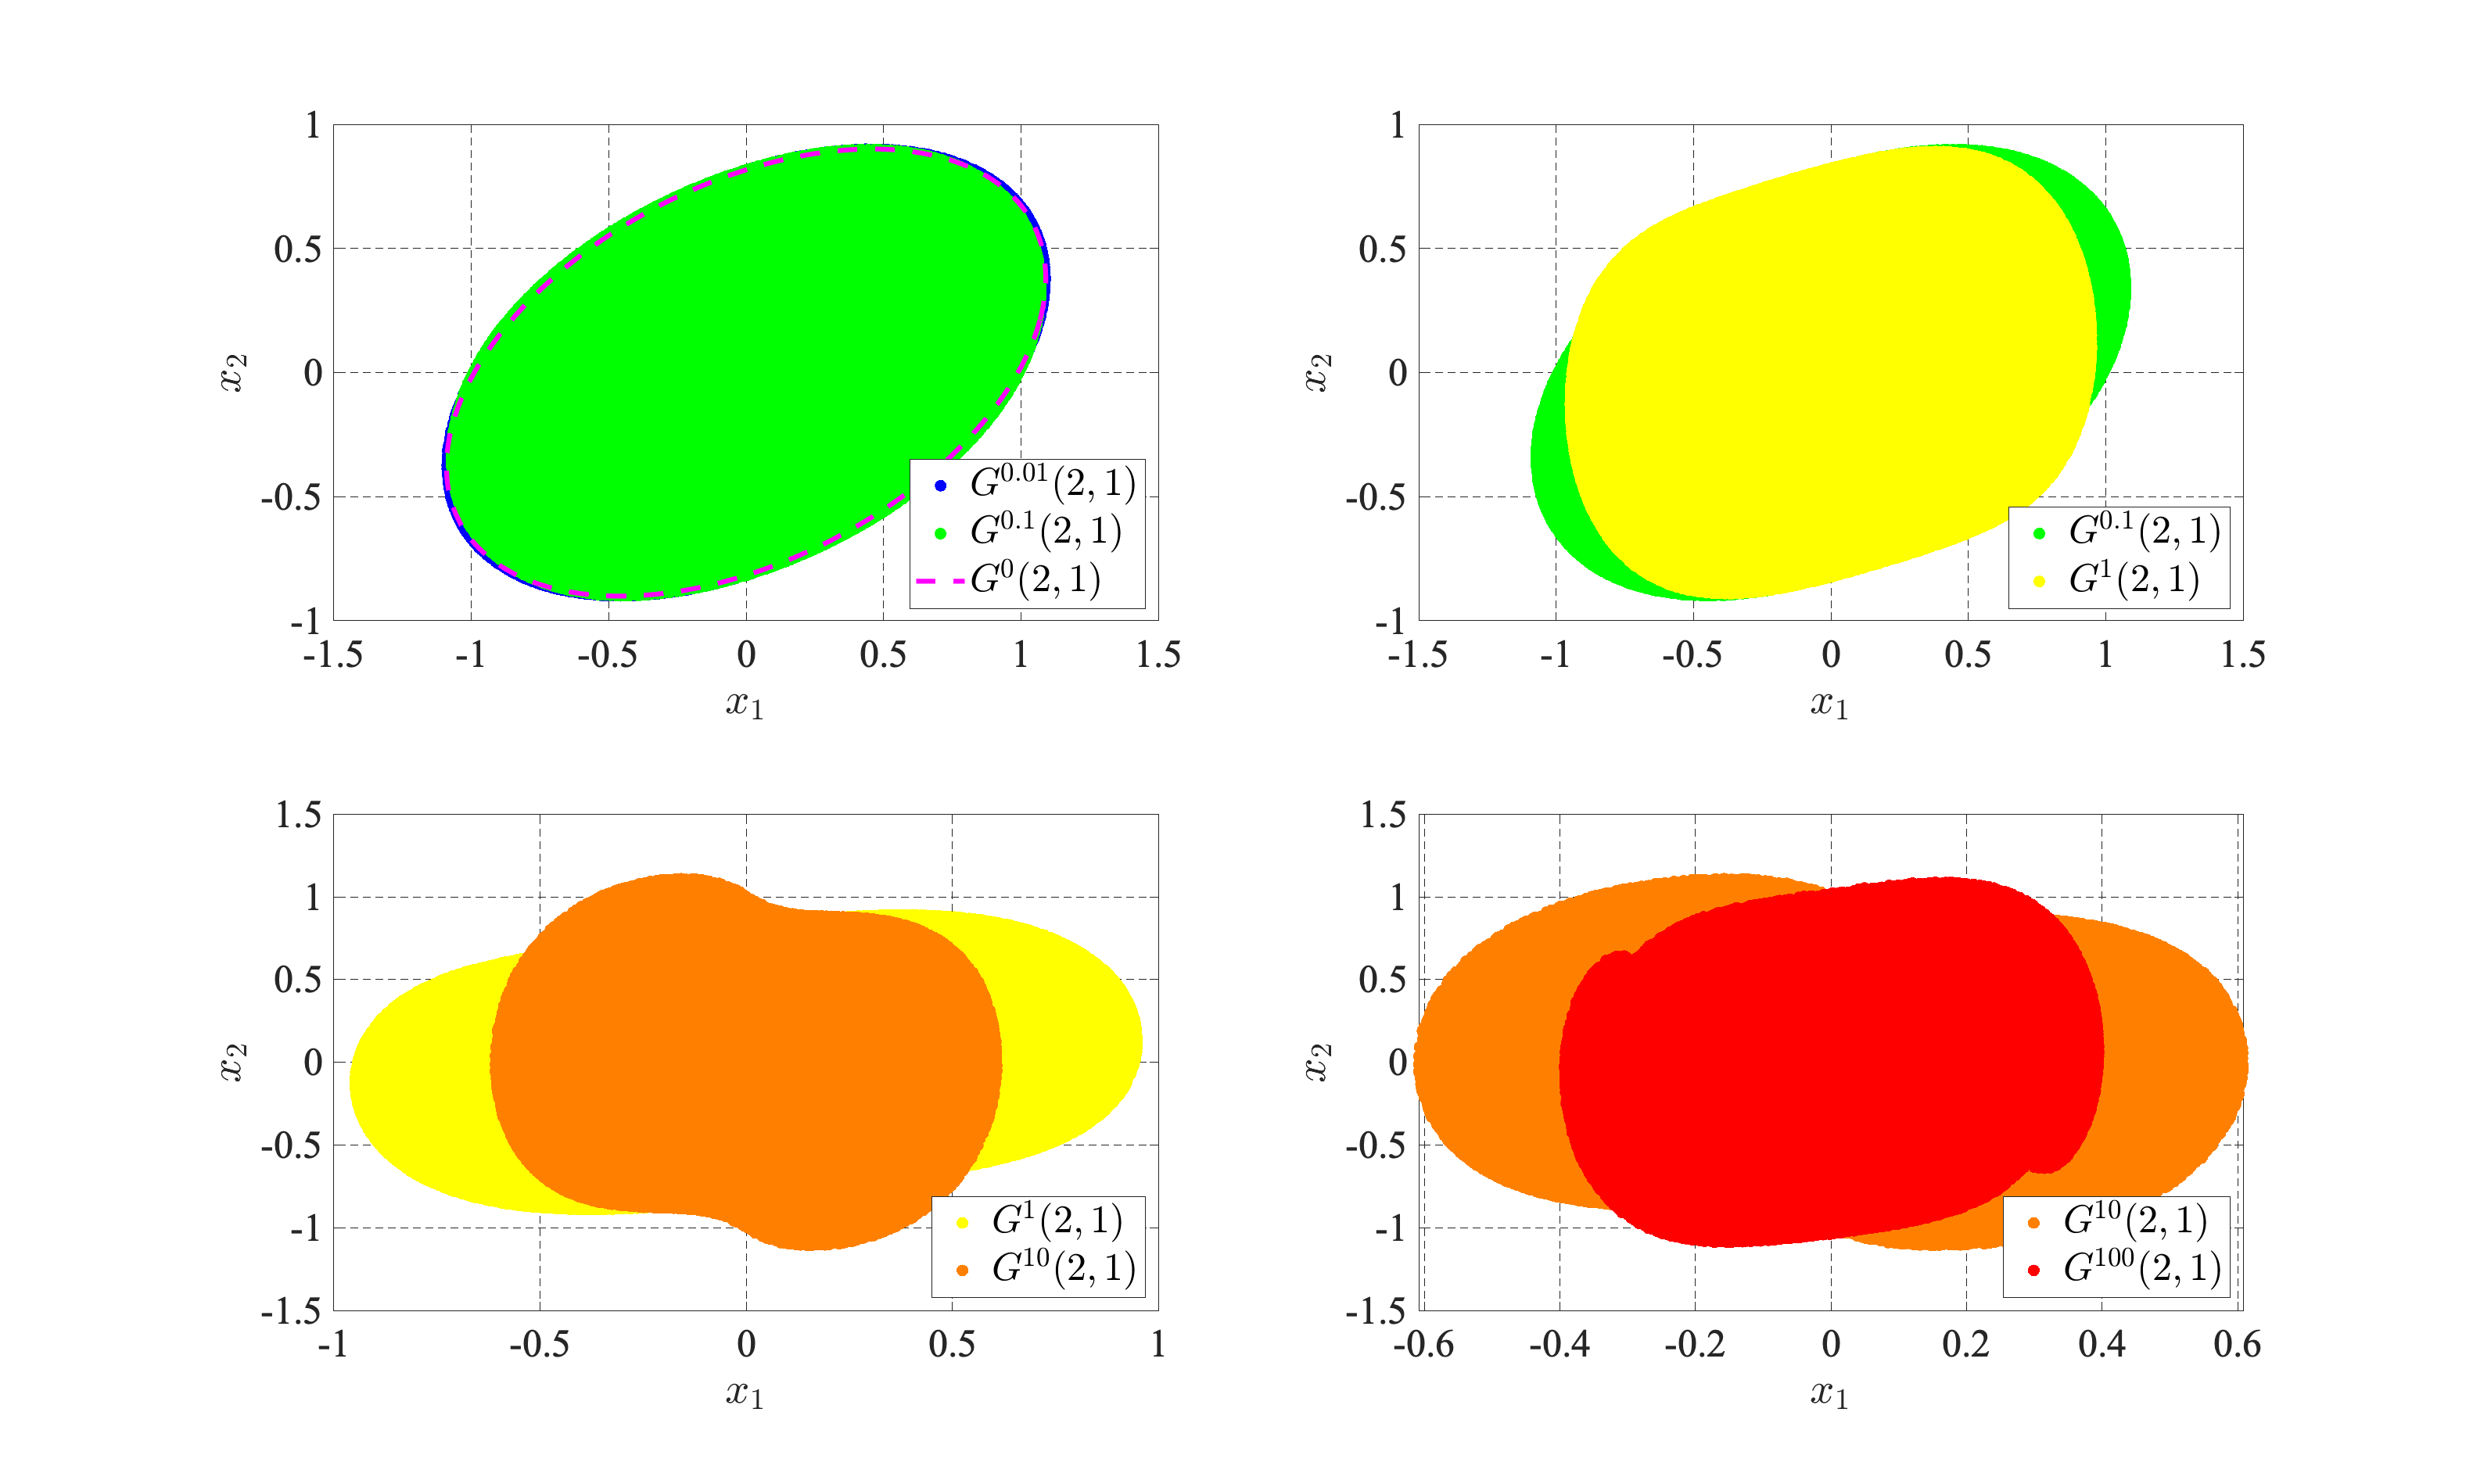
\includegraphics[width=\textwidth]{images/Osipov_QuaziDuffing.eps}}
		\caption{Множества достижимости.}
		\label{fig:Duffing}
	\end{figure}
	
	Таким образом, для системы \eqref{sec3:Duffing} выполняются требования Теоремы \ref{th:ReachableSetsConvexity}, и соответствующие множества достижимости должны быть выпуклыми для малых значений параметра. 
	Это видно на рисунке \ref{fig:Duffing}, демонстрирующем множества достижимости $G^{\varepsilon}(T,\mu)$, построенные с помощью численного метода Монте-Карло \cite{Patent,Zykov}.
	
	Видно, что множества $G^{0.01}(1,1) $ и $G^{0.1}(1,1) $ близки к множеству $G^{0}(1,1) $, которое построено для линейной системы. 
	Также видно, что при увеличении параметра $\varepsilon$ множества становятся невыпуклыми. 
	
\end{pr}  % Example (Пример)
\begin{figure}[ht]
	\centerline{
		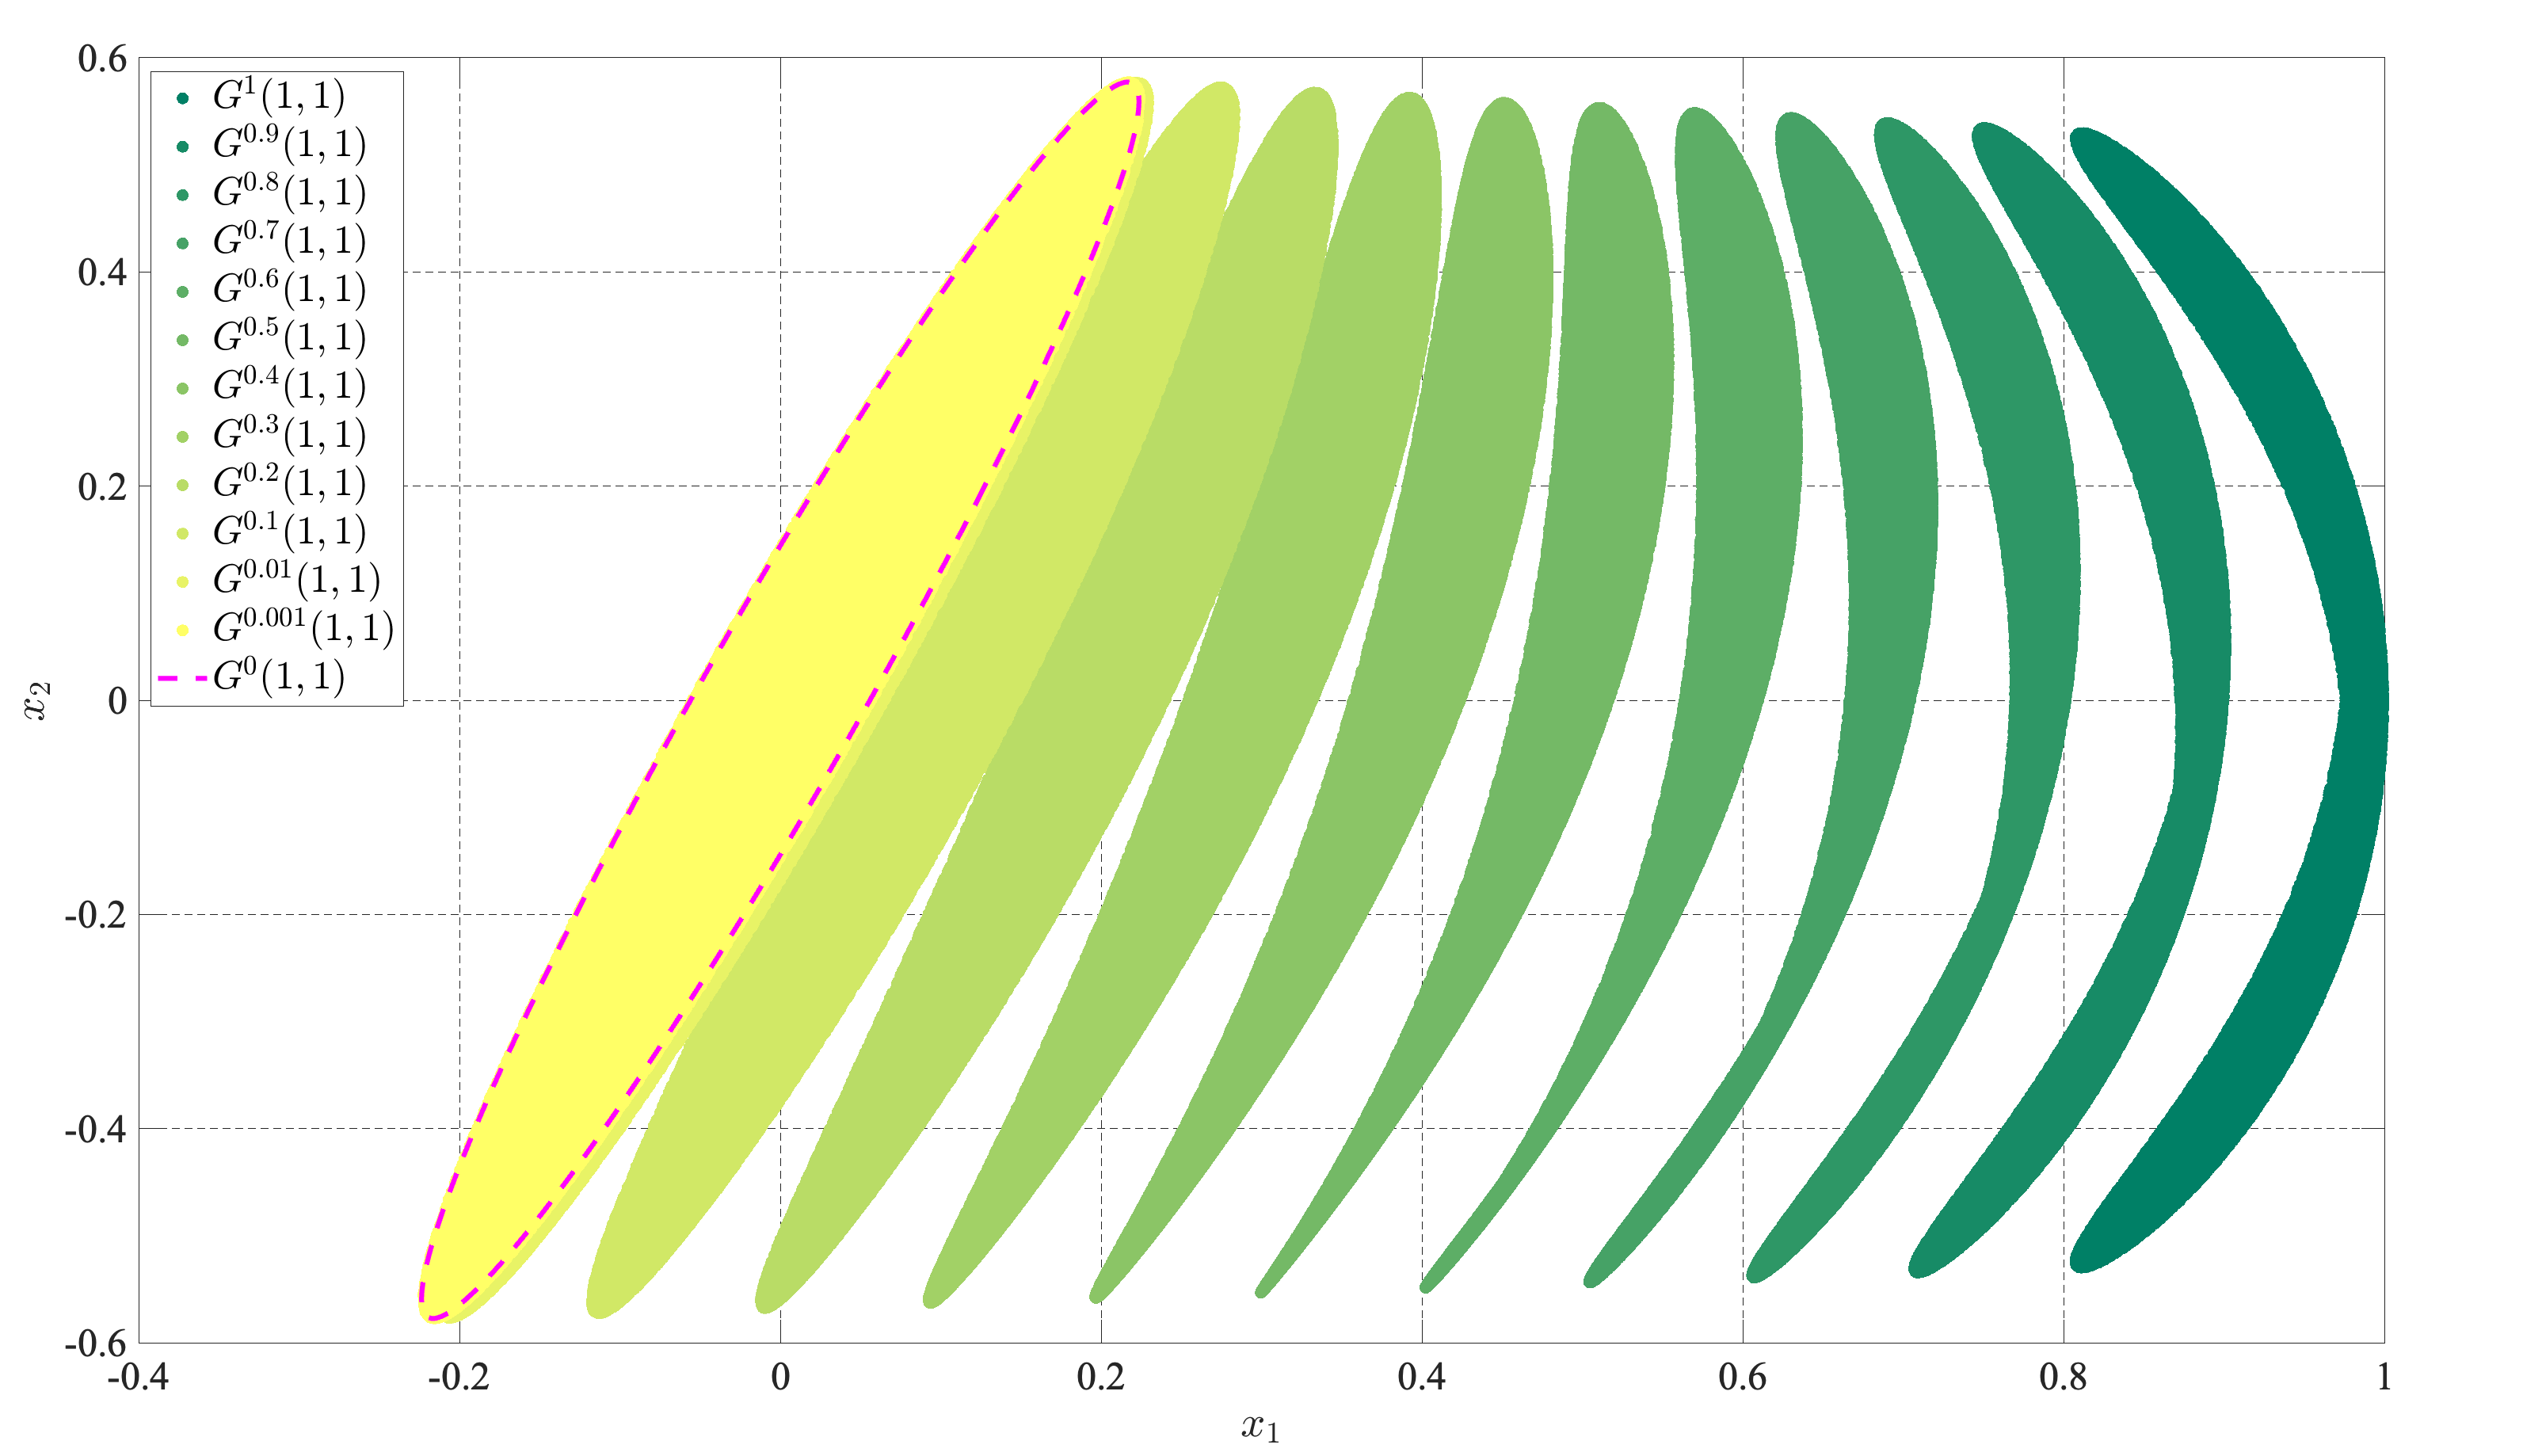
\includegraphics[width=\textwidth]{images/Osipov_QuaziDubins.eps}}
	\caption{Множества достижимости системы \eqref{Linear+Dubins}.}
	\label{fig:LinearDubins}
\end{figure}
\begin{pr}  
	Второй исследуемой системой является
	\begin{gather}\label{Linear+Dubins}
		\begin{pmatrix} 
			\dot{x}_1 \\
			\dot{x}_2 \\ 
			\dot{x}_3 \end{pmatrix} = 
		\begin{pmatrix}
			0 & 1 & 0 \\
			0 & 0 & 1 \\
			0 & 0 & 0
		\end{pmatrix}
		\begin{pmatrix} 
			x_1 \\
			x_2 \\ 
			x_3 \end{pmatrix} + 
		\varepsilon
		\begin{pmatrix}
			\cos x_3 - x_2\\
			\sin x_3 - x_3 \\
			0
		\end{pmatrix} + 
		\begin{pmatrix}
			0 \\ 0 \\ 1
		\end{pmatrix} u.
	\end{gather}
	При $\varepsilon = 0$, уравнения \eqref{Linear+Dubins} описывают линейную систему с матрицами 
	\begin{gather*}
		A = \begin{pmatrix} 0 & 1 & 0\\
			0 & 0 & 1\\ 
			0 & 0 & 1 
		\end{pmatrix}, \quad B = \begin{pmatrix}
			0\\
			0\\
			1
		\end{pmatrix},
	\end{gather*}
	а при $\varepsilon = 1$, они описываю уницикл. 
	Нелинейное слагаемое состоит из малого параметра и функции
	\begin{gather*}
		f(x) = \begin{pmatrix}
			\cos x_3 - x_2\\
			\sin x_3 - x_3 \\
			0
		\end{pmatrix}.
	\end{gather*}
	
	Начальные состояние --- нулевые, $x_1(0) = x_2(0) = x_3(0) $, ограничения на управление такие же, как и в первом примере, но мы будем рассматривать эту систему на временном интервале $0 \leqslant t \leqslant 1$.
	
	Как и в предыдущем примере, условия предположения \ref{as:right_hand_side_conditions} выполнены, что позволяет применить Теорему \ref{th:ReachableSetsConvexity}. 
	На рисунке \ref{fig:LinearDubins} показаны проекции на плоскость $(x_1,x_2)$ численно построенных множеств достижимости $G^{\varepsilon}(T,\mu)$ для системы \eqref{Linear+Dubins}. 
	
	Видно, что проекции множеств $G^{0.001}(1,1) $ и $G^{0.01}(1,1) $ близки к проекции множества $G^{0}(1,1) $, построенной для линейной системы. 
	Также видно, что проекции множеств становятся невыпуклыми при увеличении параметра $\varepsilon$. 
\end{pr}  % Example (Пример)



\end{document}